Dans cette partie, nous nous appliquerons à présenter les enjeux qui sous-tendent la production d’une indexation métier, afin de définir au mieux les besoins spécifiques des Archives nationales et les solutions envisageables pour y répondre.  Le quatrième chapitre sera donc consacré aux choix de description et de signalement des photographies numériques en fonction des contextes d’utilisation, en comparant les choix des différents services ayant travaillé sur les reportages photographiques de la Présidence, puis en mettant en regard ces expériences avec celles d’une autre institution ayant été amenée à traiter des reportages photographiques numériques : la Bibliothèque nationale de France. Dans le cinquième chapitre, nous reviendrons sur le contexte technique et institutionnel du chantier de reprise des reportages photographiques aux Archives nationales, en présentant les normes de l’archivage électronique ainsi que les solutions logiciel utilisées et leurs contraintes. Dans le sixième chapitre, nous présenterons un ensemble de solutions numériques permettant d’automatiser le traitement archivistique des reportages photographiques, en examinant leurs avantages et inconvénients.

\chapter{Des indexations différentes pour des usages différents}

Dans le chapitre précédent, nous avons présenté les enjeux liés à l’indexation des archives photographiques. Nous avons également évoqué la possibilité d'utiliser les métadonnées internes des photographies pour faciliter leur indexation dans un contexte archivistique. Pour les reportages photographiques de la Présidence de la République, ces métadonnées internes ont été produites par le service photographique. Leur utilisation dans le cadre du chantier de reprise des données présente un intérêt majeur, dans la mesure où une description à un niveau de granularité si fin est impossible à réaliser par les agents des Archives nationales dans leurs effectifs actuels. Il s’agit donc de composer avec les choix d’indexation de la cellule photographique. Cette décision cependant ne nous exempte pas d’une analyse approfondie des métadonnées descriptives renseignées par la cellule photographique et utilisées lors de la reprise des données, car pour exploiter au mieux les informations à notre disposition, il nous faut dans un premier temps les définir et mesurer le potentiel écart entre \emph{ce dont nous disposons} et \emph{ce dont nous avons besoins} dans un contexte archivistique.  Dans ce chapitre, nous présenterons les choix des différents services ayant travaillé sur les reportages photographiques de la Présidence en amont de leur versement aux Archives nationales. Dans un second temps, nous mettrons en regard ces expériences avec celle d’une autre institution ayant été amenée à traiter des reportages photographiques numériques : la Bibliothèque nationale de France. Le chapitre vise à démontrer comment le contexte de production influence non seulement la qualité de l'indexation, mais aussi les choix des sujets à indexer en fonction de besoins spécifiques. Il ne s’agit pas ici de remettre en question le choix d’utiliser l’indexation de la cellule photographique dans le cadre de la reprise des reportages aux Archives nationales. Comme mentionné précédemment, une indexation, même partielle et imparfaite, vaut mieux qu'une absence totale d’indexation. En comparant les pratiques de la cellule photographique avec celles du service des archives et de l'information documentaire de la Présidence de la République, nous nous attacherons à montrer les limites du recours à une indexation métier dans un contexte archivistique.

\section{L’indexation par la cellule photographique de la Présidence de la République}

Au sein de la cellule photographique, l’indexation est réalisée par, et pour, les agents du service. Lorsque celui-ci est doté d’un iconographe, il est chargé de la description et de l’indexation des photographies, mais dans le cas contraire ces opérations sont réalisées par les photographes eux-mêmes. Le signalement leur permet, en cas de demande adressée au service de la communication ou directement à la cellule photographique, d’identifier les fichiers y répondant au mieux. L’indexation est donc destinée à un usage interne, sans prise en compte des besoins potentiels de futurs utilisateurs extérieurs : elle a pour but de faciliter le travail des photographes en cas de demandes adressées directement à la cellule photographique ou au service de communication. 

Comme mentionné précédemment, la majorité des demandes émanent du service de la communication, du protocole, ou de conseillers. Elles consistent essentiellement en l’identification de clichés sur lesquels les demandeurs apparaissent, ou qui représentent des personnalités spécifiques, en vue d’une communication à leur sujet ou de la fabrication d’un album photographique comme cadeau diplomatique. Pour certaines communications officielles, les demandes peuvent porter sur des images du Président de la République dans des lieux particuliers ou réalisant des actions spécifiques : poignée de main, bain de foule, sourire... L’enjeu principal réside donc dans l’identification la plus précise possible des personnalités présentes, des lieux de prise de vue, ainsi que de certaines actions ou situations particulières. A première vue, les métadonnées internes descriptives semblent donc présenter un très haut niveau de précision à un niveau de granularité très fin, avec, pour certains reportages, une identification des personnalités et une légende pour chaque photographie.

Cependant, une analyse des métadonnées internes descriptives des fichiers a révélé que la qualité du travail d’indexation réalisé par la cellule photographique n’était souvent pas à la hauteur des critères de description archivistique et pouvait même comporter des erreurs, notamment dans l’emploi de la terminologie protocolaire de la Présidence de la République. Par exemple, nous pouvons observer l’utilisation indifférenciée de termes comme \enquote{visite d’état} et \enquote{visite officielle}, ainsi que l’emploi du terme \enquote{déplacement} à la place de l’appellation officielle de l’événement. De plus, le niveau de granularité de la description varie considérablement d'un reportage à l'autre : certains bénéficient d'une description détaillée pour chaque photographie, tandis que d'autres se contentent de descriptions s'appliquant à des groupes de photographies au sein d'un reportage, parfois divisés en plusieurs sections. Certains reportages ne sont décrits qu'à un niveau global, et il arrive même que certaines séries soient dépourvues de toute métadonnée descriptive interne. Au vue de ces écarts de précision et sans plus d’informations sur la méthodologie suivie par les photographes dans leur processus de description, nous pouvons nous interroger sur l’exactitude de l’indexation dans son ensemble, et en particulier celle des personnalités identifiées. 

Notre analyse a également révélé un manque de normalisation dans la terminologie utilisée pour le choix des mots-clés : non seulement une même information peut être décrite par des termes synonymes, mais ceux-ci sont parfois mal orthographiés. Les noms et fonctions des personnes identifiées peuvent également présenter des variations de graphie qui témoignent de l’absence de recours à des notices d’autorité : absence de majuscules, ordre nom/prénom interchangeable, coquilles, séparation peu explicite entre le nom et la fonction. 

En un sens, une identification incorrecte peut être préférable à une absence totale d’indexation. Avec les outils de recherche d’images disponibles sur internet, il est souvent plus simple de vérifier si la personne mentionnée dans les métadonnées descriptives correspond bien à celle recherchée, que de parcourir l’ensemble des fichiers d’un reportage à la recherche d’un cliché identifiable. Par ailleurs, en l’absence d’un contrôle de la qualité de l’indexation par un autre service de l’Élysée, les photographes restent les seuls responsables des métadonnées qu’ils produisent. Ce contexte de production et d’utilisation des métadonnées en vase clos explique les éventuels manques de précision : la qualité des métadonnées internes dépend en grande partie de la rigueur des photographes et iconographes, qui a pu varier en fonction des capacités et des besoins du service. De plus, ces imprécisions sont tout à fait compréhensibles dans la mesure où la description et l'indexation ne font pas partie des missions des photographes mais relèvent des compétences d'iconographes ou de documentalistes. Il n'en demeure pas moins que ces imprécisions rendent le signalement peu efficace et plus difficile à appréhender pour les services qui souhaitent l'exploiter dans des contextes différents. Au Archives nationales, l'indexation des reportage n'est pour le moment pas destinée à orienter les usagers, le fonds n'étant pas librement communicable. Elle doit permettre aux archivistes de naviguer plus facilement dans le fonds afin de répondre aux demandes de communication des usagers.

\section{Indexation par la mission archives}

Avant d’être versés aux Archives nationales, les reportages photographiques sont traités et archivés par le service des archives et de l'information documentaire de la Présidence de la République dans une base de données Cindoc, un système de gestion électronique de documents. Lorsque les reportages sont extraits en vue de leur versement aux Archives nationales, ils sont accompagnés d’un fichier au format \gls{csv} généré par la base de données Cindoc. Ce fichier offre une description du reportage, incluant le numéro du reportage, l’intitulé, les dates de début et de fin, ainsi qu’une série de mots-clés thématiques. Lors de la reprise des reportages, nous avions initialement envisagé d’utiliser les termes d'indexation issus de ces fichiers CSV pour une description au niveau du reportage. Cependant, nous avons finalement choisi de nous appuyer sur les descriptions fournies par la cellule photographique, qui permettent une indexation plus granulaire, au niveau de chaque photographie. Il nous semble néanmoins important de présenter ces exports CSV pour mieux comprendre le travail réalisé par les archivistes de l’Élysée, les exigences auxquels ils répondent, et démontrer ainsi l’intérêt d’intégrer ces documents au chantier de reprise des données.

Créé en 1998, le produit Cindoc est un système de gestion documentaire et de gestion électronique de documents (GED). Il permet de gérer, stocker et diffuser tout type de fonds documentaire et est très largement utilisé par les institutions patrimoniales, notamment les services d’archives chargés de l’archivage intermédiaire. Doté d’outils d’indexation et de recherche puissants, il dispose également de fonctions spécifiques à la gestion d’un fonds d’images. Il permet la création de thésaurus normés\footnote{Normes ISO 2788 et 5964} et une indexation adaptée aux différents contextes de production, notamment avec du texte libre et la possibilité de créer autant de champs d’identification qu’on le souhaite\footnote{Présentation de Cincom CinDoc, \url{https://www.cincom.com/pdf/un-acteur-historique.pdf}, consulté le 15 août 2024.}. 

La base de donnée CinDoc est renseignée par les archivistes de l’Élysée et fournit des informations de description et d’analyse pour chaque reportage. La liste des reportages est créée à partir de l’agenda officiel du Président de la République.  Le signalement réalisé par les archivistes est le fruit de réflexions reflétant les demandes de communications qui ont pu être faites, afin d’y répondre au mieux par la suite. L’indexation reprend des éléments thématiques, iconographiques et géographiques, ainsi que les personnes identifiées sans doute possible. En général, les demandes sont adressées à la cellule photographique. Celle-ci se tourne alors vers les archivistes qui lui fournissent le ou les reportages correspondant dans leur ensemble, la cellule photographique procède ensuite à la sélection des clichés. Lorsqu’une demande précise est adressée au service des archives par un autre service, les archivistes prennent le temps de regarder les fichiers afin de choisir les clichés correspondant à la demande. Parmi les demandes de communication internes, les plus fréquentes sont les demandes d’albums photographiques comme cadeau protocolaire : d’après Evelyne Van Den Neste, les services produisent près d’un album par mois. Dans l’ensemble, les demandes peuvent émaner de la cellule communication, du service du protocole, de la cellule diplomatique ou des conseillers, parfois pour des demandes privées. Les archivistes de l’Élysée reçoivent des demandes de communication similaires à celles envoyées à la cellule photographique, par exemple le Président dans une pièce spécifique de l’Élysée, le Président en présence d’un chien, le protocole suivi lors de la dernière visite d’un Président français à Jérusalem. Dans le cas de ce dernier exemple, il s’agissait de vérifier si les prédécesseurs du Président avaient porté une kippa lors d’une visite du mur des Lamentations.

Les mots-clés produits par le service des archives sont le fruit d’une méthodologie rigoureuse et de multiples vérifications, ils sont donc plus fiables dans leur ensemble que ceux fournis par les métadonnées internes des fichiers. Les noms propres se présentent toujours sous la même forme (Nom Prénom), l’absence de caractères spéciaux facilite la recherche, et le vocabulaire employé est normalisé. Cependant, l’indexation des archivistes présente ses propres spécificités qui la rendent peu pertinente pour un signalement dans le système d’archivage électronique des Archives nationales. Afin d’éviter les erreurs d’identification et pour garantir le respect du vocabulaire normalisé, ne sont mentionné que les termes qui ont pu être vérifiés à l’aide de l’agenda ou d’une première analyse des photographies. La quantité de clichés ne permettant pas une analyse exhaustive de chaque reportage, l’indexation est nécessairement moins riche que celle de la cellule photographique : moins de mots-clés descriptifs, moins de noms de personnes présentes… L’indexation est divisée en quatre catégories thématiques : « CLE », « DES », « PER », « GEO ». 
\begin{itemize}
	\item La section « CLE » contient les mots-clés généraux associés à l’ensemble du reportage. 
	\item La section « DES » contient des termes permettant de décrire le décor ou les action visibles sur les photographies du reportage. 
	\item La section « PER » liste les personnes identifiées.
	\item La section  « GEO » contient les noms de lieux liés au reportage, qu’il s’agisse du lieu où s’est déroulé le reportage ou de lieux liés thématiquement au sujet (pays d’où sont originaires les personnalités présentes, lieux dont il a été question au cours d’une intervention…).
\end{itemize}

A titre d'exemple, les descriptions issues du fichier CSV de la base CinDoc pour les trois premiers reportages de la mandature de François Hollande sont présentées dans un tableau sur la page suivante. 
\newpage

\begin{table}[h]
	\begin{tabular}{|p{4cm}|p{2.5cm}|p{2.5cm}|p{2.5cm}|p{2.5cm}|}
		\hline
		\rowcolor{pastelyellow-dark}
		\textbf{OBJET} & \textbf{CLE} & \textbf{DES} & \textbf{PER} & \textbf{GEO} \\
		\hline
		\rowcolor{pastelyellow}
		Cérémonie d'investiture de François Hollande, Président de la République, Palais de l'Elysée & ceremonie, ceremonie d'investiture, investiture , passation de pouvoir & tapis rouge, cour d'honneur, poignee de main, sourire, ceremonie & Sarkozy Carla, Sarkozy Nicolas, Hollande François, Trierweiler Valerie & Palais de l'Elysee, Paris \\
		\hline
		\rowcolor{pastelyellow}
		Cérémonie d'hommage au soldat inconnu à l'Arc de Triomphe, Paris, 15 mai 2012. & deplacement, ceremonie, hommage, soldat inconnu & poignee de main, salut au drapeau, salut de la main, cour d'honneur, tapis rouge, motocyclette, pluie & & Paris, Arc de Triomphe\\
		\hline
		\rowcolor{pastelyellow}
		Déjeuner avec des anciens Premier ministre, Palais de l'Elysée, Paris, 15 mai 2012. & dejeuner, ministre & table, dejeuner, dejeuner de travail & Trierweiler Valerie, Morelle Aquilino, Fabius Laurent, Jospin Lionel & Palais de l'Elysee \\
		\hline
	\end{tabular}
	\caption{Intitulés et mots-clés des trois premiers reportages de la mandature de François Hollande tels qu'ils sont renseignés dans l'export au format CSV de la base de données CinDoc.}
\end{table}

Les mots-clés géographiques en particulier posent problème, car aucune distinction n'est faite entre les lieux de prise de vue et les lieux connectés thématiquement au reportage. L'information correspondant au lieu de prise de vue est présente à deux reprises dans chaque entrée du fichier CSV, mais n'est jamais caractérisée : elle est indiquée avant la date dans l'intitulé du reportage, et de manière indifférenciée dans la catégorie de mots-clés \enquote{GEO}.  L'exploitation de ce signalement serait particulièrement difficile : elle nécessite de trouver un moyen de caractériser dans les deux cas l'information \enquote{lieu de prise de vue du reportage}. Cette opération se complique encore davantage dans le cas des reportages \enquote{itinérants} qui se sont déroulés dans plusieurs lieux différenciés. Une analyse des autres mots-clés cependant nous renseigne sur le type de clichés attendu par les services sollicitant les archivistes de l'Élysée : poignée de main, sourire, tapis rouge, salut de la main... Il est aisé d'imaginer dans quelle mesure ces mots-clés permettent de faire ressortir les reportages contenant des photographies pouvant intéresser les services du protocole ou la cellule communication. Nous observons cependant que les noms des personnes présentes ne sont pas toujours renseignés, comme c'est le cas pour la cérémonie d'hommage au soldat inconnu. Ainsi, malgré le travail de recherche permettant de garantir l'exactitude de l'indexation produite par le service des archives, cette méthode n'est pas en adéquation avec des demandes de recherche plus généralistes ou s'inscrivant dans une démarche de recherche historique.

\section{Etude de cas : l'indexation des photographies numériques à la Bibliothèque nationale de France}

Les reportages photographiques de la Présidence de la République et des Services du Premier Ministre constituent un exemple unique de fonds quasi-exclusivement constitué de photographies nativement numériques aux Archives nationales. Afin de prendre du recul et d’élargir notre perspective, nous avons exploré comment d’autres institutions patrimoniales ont pu gérer des versements similaires. L’objectif était de savoir si elles avaient rencontré des problèmes analogues et comment elles les avaient résolus. Dans ce cadre, nous avons rencontré Alix Bruys, conservatrice à la Bibliothèque nationale de France (BnF) et responsable des acquisitions et dons numériques. Elle a partagé avec nous son expérience de collecte de reportages photographiques nativement numériques pour le projet \enquote{Radioscopie de la France : regards sur un pays traversé par la crise sanitaire} en 2022. Au regard du travail effectué sur les reportages photographiques de la Présidence, il ressort de cette expérience un rapport très différent à l'indexation, bien que les réflexions qui en ont découlé présentent des similitudes notables avec celles menées aux Archives nationales.

Le cas de la BnF est particulièrement intéressant car il s’agit d’une institution qui a pu commander ces reportages, anticipant ainsi les besoins en matière de description et les problématiques techniques associées. Nous avons examiné les métadonnées qui avaient été demandées, la méthode proposée, ainsi que les résultats obtenus. Dans le contexte d'une commande aussi spécifique, il nous semble également intéressant d'évaluer dans quelle mesure les photographes se sont impliqués dans ce processus et comment la BnF a intégré ces reportages dans son catalogue. Cette étude de cas pourrait nous offrir un angle unique pour comprendre les méthodes de travail des photographes et leur relation à l’indexation dans le contexte de la photographie numérique.

\subsection*{Histoire d'une collecte : la commande de reportages photographiques à la Bibliothèque nationale de France}
Le traitement de reportages photographiques numériques à la BnF commence bien avant le projet de \enquote{Radioscopie de la France} en 2022. C'est le département des Arts du spectacle qui est à l'origine des premières collectes de ce type. Les collections de ce département permettent d'étudier la totalité des formes des arts de la scène et du spectacle de rue en confrontant des fonds de natures différentes : documents écrits, documents iconographiques, images animées, objets scéniques... La bascule de l'argentique vers le numérique s'effectue progressivement à la BnF entre 2005 et 2010, les photographes documentaires arrêtant petit à petit de fournir des négatifs et diapositives pour ne plus produire que des photographies numériques. Les photographes, intéressés principalement par le rendu visuel et non par la technique numérique, se penchent peu sur les informations portées par les fichiers. 

La situation évolue entre 2021 et 2022 lorsque le département des Estampes et de la photographie se dote d’un service consacré à la photographie numérique. A l'époque, dans le cadre du plan gouvernemental de soutien à la filière presse, le ministère de la Culture a confié à la Bibliothèque nationale de France la mise en œuvre d’une grande commande photographique, \enquote{Radioscopie de la France : regards sur un pays traversé par la crise sanitaire}, destinée aux photojournalistes. Après deux appels à projet, 200 photojournalistes ont été sélectionnés. Les \oe{}uvres produites ont ensuite été intégrées aux collections de la BnF, au sein du département des Estampes et de la photographie. Les photojournalistes devaient s'engager à fournir 10 tirages et un reportage numérique, sans contrainte volumétrique. Les projets devaient permettre de dessiner un portrait de la France, sans nécessairement se concentrer sur la crise sanitaire, à partir des 10 tirages. Les reportages numériques en revanche devaient permettre de suivre les photojournalistes sur le terrain, en présentant le contexte de production des tirages\footnote{Pour plus d'informations, voir le site de la grande commande : \url{https://www.bnf.fr/fr/grande-commande-photojournalisme}.}.

\subsection*{Elaboration de spécifications pour le signalement et la préservation des reportages}

Le caractère commandé de ce versement plutôt que de simple collecte, confère à l'institution réceptrice le pouvoir de définir des exigences précises quant au contenu, et d'imposer des spécifications techniques pour les reportages photographiques. Certaines caractéristiques techniques des reportages versés ont donc pu être anticipées dès la phase de production des images. La BnF a ainsi rédigé une documentation détaillant les formats requis ainsi que les caractéristiques du flux d’images attendu. Cette documentation inclut notamment une sélection des champs de métadonnées IPTC à renseigner, afin de faciliter les futures analyses de données en masse à des fins de recherche. 

Le format demandé est du TIFF (version 6, sans compression), bien que le JPEG soit toléré si les photographies avaient été produites directement dans ce format, les conversions de JPEG vers TIFF n'étant pas recommandées. Les photographies couleur devaient être encodées en RVB, avec une profondeur de 24 bits, et les images en niveaux de gris avec une profondeur de 8 bits par couche. Ces choix sont dictés par la compatibilité avec les images diffusées sur Gallica, la plateforme numérique de la BnF. Cependant, cet outil, initialement conçu pour des numérisations de documents physiques, n'est pas optimisé pour les images nativement numériques. Ainsi, dans le système actuel, une copie de visualisation est produite pour l'accès public, mais les métadonnées ne sont pas récupérables directement sur l’image diffusée. Le système SPAR (Système de Préservation et d'Archivage Réparti)\footcite{sparBNF} génère une version de diffusion pour les documents consultables sur Gallica, selon les règles de communicabilité.

Les spécifications élaborées par la filière \enquote{Acquisitions et dons de documents numériques} prévoient 5 métadonnées IPTC obligatoires et 4 optionnelles. Les cinq champs obligatoires correspondent au titre, au nom du photographe, à la légende de la photographie, au lieu de prise de vue, et le champ de crédit. Les quatre métadonnées optionnelles sont : le type de source numérique, les mots-clés, l'identification des personnes représentées et l'identifiant du reportage attribué par le photographe. Les spécifications précisent également les champs IPTC réservés aux besoins de la BnF et ne devant donc pas être renseignés, tous liés à l'identification du fournisseur de l'image\footcite{speacqbnf}. Au moment de la commande des reportages, la BnF n’avait toutefois pas encore établi de correspondance formelle (mapping) entre le standard \gls{InterMARC} utilisé par Gallica et les métadonnées IPTC. L'absence de correspondance entre les métadonnées IPTC et les champs en InterMARC peut poser des défis supplémentaires pour l’intégration des images dans le catalogue de la bibliothèque.

Les deux tableaux à la page suivante sont extraits des spécifications de la BnF et indiquent les métadonnées obligatoires et optionnelles, ainsi que des descriptions précises de la forme et du type d'information attendus. Cette dernière précision est très importante, car les noms des champs de métadonnées ne sont pas toujours explicites et peuvent donner lieu à plusieurs interprétations. Nous pouvons rappeler, à titre d'exemple, l'indexation dite \enquote{géographique} du service des archives de la Présidence qui regroupait le lieu de prise de vue et les lieux liés thématiquement au reportage. 

\newpage
\begin{figure}[h]
\begin{adjustbox}{width = \textwidth, center}
	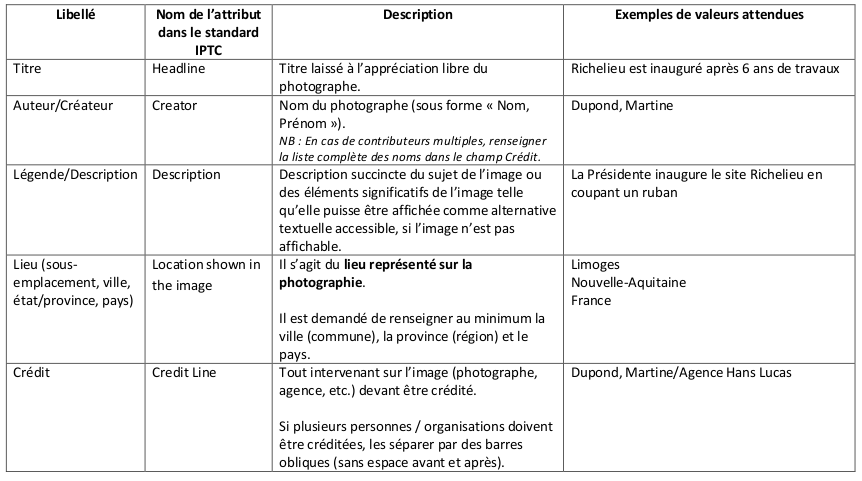
\includegraphics{./img/spe_iptc_bnf.png}
\end{adjustbox}
\caption{Liste des métadonnées IPTC obligatoires, Source : BnF, Spécifications des photographies nativement numériques}
\end{figure}

\begin{figure}[h]
	\begin{adjustbox}{width = \textwidth, center}
		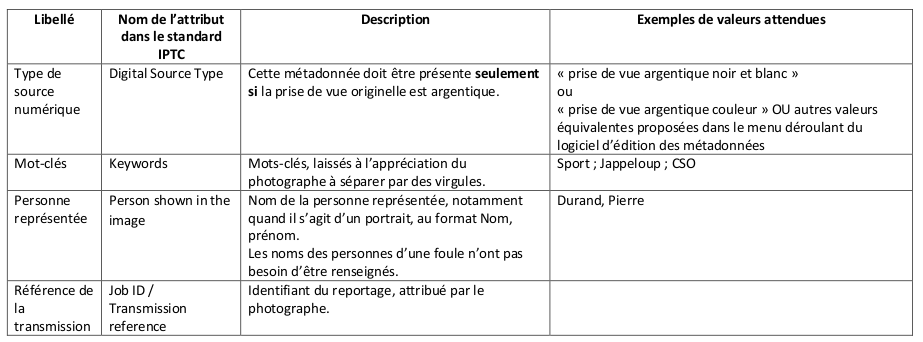
\includegraphics{./img/opt_iptc_bnf.png}
	\end{adjustbox}
	\caption{Liste des métadonnées IPTC optionnelles, Source : BnF, Spécifications des photographies nativement numériques}
\end{figure}
\newpage



\subsection*{Des exigences peu respectées}

Cependant, à l'issue de la collecte de l'ensemble des reportages, il s'est avéré qu'environ un tiers des photojournalistes n'ont pas respecté les spécifications, tant pour les métadonnées internes que pour les formats de fichier. Ainsi, plusieurs photographes ont envoyé des images au format TIFF 48 bits au lieu de 24 bits. De plus, beaucoup de champs de métadonnées n'ont pas été remplis, ou l'ont été sans suivre les recommandations de la BnF. 

Pour analyser les métadonnées renseignées, les équipes de la BnF se sont dotées du logiciel de visualisation d'images XnView, également utilisé aux Archives nationales, et qui permet d'afficher le contenu visuel ainsi qu'un éventail très large des métadonnées internes. Cependant, ce mode de visualisation ne permet pas d'afficher les métadonnées d'un ensemble d'images. Au cours de notre échange avec Alix Bruys, celle-ci nous expliquait que l'équipe en charge du traitement des photographies numériques avait engagé des réflexions pour mettre en place une méthode d'analyse plus systématique et plus massive des métadonnées internes à l'aide de l'application Exiftool\footnote{Voir le site de l'application : \url{https://exiftool.org/}}. Il s'agit de l'une des applications les plus performantes pour la lecture, l'écriture et l'édition des métadonnées internes d'images numériques, c'était donc également sur elle que s'était porté notre choix pour l'analyse des reportages photographiques de la Présidence de la République. Nous reviendrons sur le fonctionnement de cette application plus en détail dans le sixième chapitre de ce mémoire. 

Une différence notable avec le traitement des reportages photographiques de la Présidence de la République aux Archives nationales réside dans l'usage prévu des métadonnées internes : dans le cas de la BnF, celles-ci ne sont pas destinées au signalement, mais sont uniquement envisagées pour de futures études sur le fonds. Dans le processus d’acquisition de la BnF, la création des notices se fait manuellement, sans processus d'exploitation automatisée des métadonnées internes. Celles-ci étant plutôt destinées à des exploitations ultérieures dans un contexte de recherche scientifique, il n'a pas été demandé aux photojournalistes d'amender les fichiers qui ne respectaient pas les spécifications : l'ensemble des reportages a été accepté tel que versé. Le travail de description et d'indexation requis est conséquent, et dépend grandement de celui réalisé en amont par le photojournaliste. Cependant, il est sans commune mesure avec le travail de description requis pour les reportages de la Présidence de la République : s'il est long et laborieux de procéder au signalement des 200 reportages du projet \enquote{Radioscopie de la France : regards sur un pays traversé par la crise sanitaire}, il l'est d'autant plus pour les près de 8000 reportages de la Présidence de la République, réalisés entre la seconde mandature de Jacques Chirac et celle de François Hollande.
\\

Pour comprendre les écarts constatés entre les spécifications définies par la BnF et les résultats obtenus, plusieurs facteurs peuvent être évoqués. Il est possible que certains photographes n’aient pas disposé des outils nécessaires pour transformer leurs fichiers dans le format requis ou que les appareils utilisés n'aient pas permis produire directement le format attendu. Les photographes ont pu utiliser des applications qui ne prenaient pas en charge les champs de métadonnées spécifiés, ou n’étaient peut-être pas familiers avec les différents schémas de métadonnées (EXIF, XMP, IPTC). Par ailleurs, il est envisageable que certains photojournalistes aient pensé qu'envoyer des fichiers dans une qualité supérieure serait préférable, sans avoir conscience des contraintes spécifiques imposées par la diffusion sur Gallica, ni de l’impact sur l’espace de stockage. Si les raisons d'être des spécifications techniques n’ont pas été explicitement communiquées, les photographes ont pu ne pas en comprendre l'importance.

Ces interrogations mettent en lumière un problème similaire à celui rencontré lors du traitement des reportages de la Présidence de la République. Lorsque les photographes ou producteurs se concentrent uniquement sur une description ou une indexation qui répond à leurs besoins immédiats, sans avoir une connaissance ou une compréhension claire des besoins des futurs utilisateurs, ils peuvent ne pas les prendre en compte. Cette étude de cas a démontré que, même lorsque ces besoins sont clairement exprimés en amont, comme dans le cas de la BnF, cela ne garantit pas que les photographes respecteront scrupuleusement les consignes. Nous ne pouvons bien sûr pas exclure l'hypothèse d'une simple négligence, dans la mesure où ces descriptions n'impactent en rien le travail du photographe. De plus, le niveau de technicité exigé par les processus de migration de format ou de renseignement des métadonnées internes peut ne pas être acquis par certains photographes.

De manière plus générale encore, ces exemples nous poussent à nous interroger sur l'implication des services producteurs dans le processus archivistique. Si les besoins liés à une gestion pérenne des documents numériques étaient pris en compte dès leur production, bien des obstacles rencontrés lors de la reprise des reportages photographiques auraient pu être évités. Cela nécessiterait cependant une évolution des politiques de gestion documentaire à l'échelle des institutions, qui devraient alors implémenter les principes d'interopérabilité des données produites. Tant que ce ne sera pas le cas, nous ne pouvons attendre des services producteurs qu'ils se conforment à des exigences extérieures à leurs propres besoins. Il convient alors de s'adapter aux contraintes propres aux documents versés en cherchant, lorsque cela est possible, des solutions palliatives. L'utilisation des descriptions réalisées par la cellule photographique n'est pas pour autant inadaptée au signalement dans un contexte archivistique. Toutefois, il est important de rappeler qu'il s'agit d'une solution imparfaite, une béquille destinée à pallier les lacunes induites par les contraintes spécifiques à la reprise des reportages photographiques de la Présidence : notamment le manque de temps et de ressources humaines. Cette approche revient à fusionner l'objet numérique et sa description, les métadonnées internes faisant partie intégrante des informations embarquées dans l'archive photographique.


